\section{Task 1: Theory}
\subsection*{a)}
Opening can be defined as: 
\begin{equation}
    f \circ b = (f \ominus b) \oplus b
\end{equation}
Or, first applying an erosion, then applying a dilation using the same structuring element on the image. 

Closing can be defined as: 
\begin{equation}
    f \bullet b = (f \oplus b) \ominus b
\end{equation}
Or, first applying a dilation, then applying a erosion using the same structuring element on the image. 

After the first opening or closing, applying more openings or closings will not have any effect on the same image as you will inevitably erode and dilate the same shape each time. 

\subsection*{b)}
This is because the edge detection (and derivatives in general) enhance noise, making it virtually impossible to detect edges on a noisy image. Therefore it would be necessary to apply smoothing to the image, to remove noise (and preserves the edges), before we can detect any edges. See \cref{fig:noisy_edge}, which illustrates how noise is amplified when derivated. 

\begin{figure}[]
    \centering
    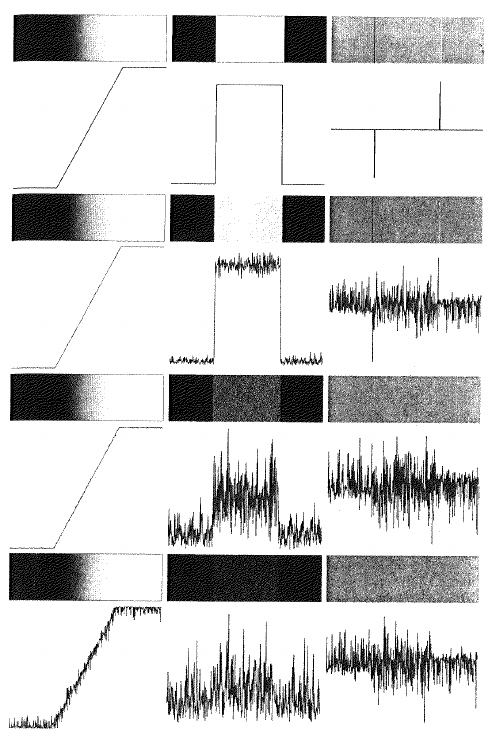
\includegraphics[width=1.00\textwidth]{figures/noisy_edge.png}
    \caption{Ramp edge with different levels of noise. From figure 10.7 Digital Image Processing. }
    \label{fig:noisy_edge}
\end{figure}

\subsection*{c)}
Rather than using a single threshold, we use two thresholds, one lower and one higher. Anything larger than the higher is marked as an edge, and anything below the lower is marked as not an edge. Those between these threshold can be seen as weak edges, and is marked as an edge if there is a strong edge next to it. 

\subsection*{d)}
We use hysteresis thresholding instead of a single threshold because it is difficult to get a single useful value for thresholding. If the value is too high, the weak edges (as mentioned in c)) would be ignored, and if the value is too low, then unwanted values (noise) would be counted as real edges. Hysteresis thresholding gives us a decent way to include likely edges (weak edges close to strong edges). 

\subsection*{e)}
Reflecting $B$ has no effect. Centre has been highlighted with bold. Values outside A was handled as zeros. 

\begin{align*}
    A &= \begin{bmatrix}
        0 & 0 & 0 & 0 & 0 & 0 \\
        1 & 0 & 0 & 0 & 1 & 0 \\ 
        0 & 1 & 1 & 1 & 0 & 0 \\ 
        1 & 0 & 0 & 0 & 1 & 0 \\ 
        0 & 0 & 1 & 0 & 0 & 0 \\ 
        0 & 0 & 0 & 0 & 0 & 0 
    \end{bmatrix} \\ 
    B &= \begin{bmatrix}
        1 & \mathbf{1} & 1
    \end{bmatrix} \\ 
    A \oplus B &= \begin{bmatrix}
        0 & 0 & 0 & 0 & 0 & 0 \\
        1 & 0 & 0 & 0 & 1 & 0 \\ 
        0 & 1 & 1 & 1 & 0 & 0 \\ 
        1 & 0 & 0 & 0 & 1 & 0 \\ 
        0 & 0 & 1 & 0 & 0 & 0 \\ 
        0 & 0 & 0 & 0 & 0 & 0 
    \end{bmatrix} \oplus \begin{bmatrix}
        1 & \mathbf{1} & 1
    \end{bmatrix} \\ 
    &= \begin{bmatrix}
        0 & 0 & 0 & 0 & 0 & 0 \\
        1 & 1 & 0 & 1 & 1 & 1 \\
        1 & 1 & 1 & 1 & 1 & 0 \\ 
        1 & 1 & 0 & 1 & 1 & 1 \\ 
        0 & 1 & 1 & 1 & 0 & 0 \\ 
        0 & 0 & 0 & 0 & 0 & 0 
    \end{bmatrix}
\end{align*}
